% !TEX TS-program = pdflatex
\documentclass[11pt]{article}

% -------------------- Packages --------------------
\usepackage[a4paper,margin=1in]{geometry}
\usepackage{amsmath,amssymb}
\usepackage[T1]{fontenc}
\usepackage{lmodern}
\usepackage{xcolor}
\usepackage{tcolorbox}
\tcbuselibrary{skins,breakable}
\usepackage{enumitem}
\usepackage{hyperref}
\usepackage{tikz}
\usetikzlibrary{calc,patterns,angles,quotes,intersections}

\pagestyle{empty}

% -------------------- Dark Theme Colors --------------------
\definecolor{bg}{HTML}{000000}
\definecolor{pairbg}{HTML}{121212}
\definecolor{solbg}{HTML}{0A0A0A}
\definecolor{border}{HTML}{2A2A2A}
\definecolor{text}{HTML}{FFFFFF}
\definecolor{muted}{HTML}{C9CDD3}
\definecolor{gold}{HTML}{FFD700}
\definecolor{green}{HTML}{4ADE80}
\definecolor{cyan}{HTML}{38BDF8}

\pagecolor{bg}
\color{text}

\hypersetup{
  colorlinks=true,
  linkcolor=cyan,
  urlcolor=cyan
}

\setlength{\parindent}{0pt}
\setlength{\parskip}{10pt}

\setlist[itemize]{left=1.4em,itemsep=6pt,topsep=6pt}
\setlist[enumerate]{left=1.6em,itemsep=4pt,topsep=4pt}

% -------------------- tcolorbox Base --------------------
\tcbset{
  enhanced,
  breakable,
  arc=12pt,
  boxrule=0.8pt,
  left=16pt,right=16pt,top=12pt,bottom=12pt
}

\newtcolorbox{QAPair}[1]{%
  colback=pairbg,
  colbacklower=solbg,
  colframe=border,
  coltext=text,
  title=\textcolor{gold}{\bfseries #1},
  fonttitle=\bfseries,
  coltitle=text,
  segmentation style={draw=border, dashed, line width=0.6pt},
}

\newtcolorbox{QuickBox}{%
  colback=pairbg,
  colframe=cyan,
  coltext=text,
  fontupper=\color{text},
  borderline north={4pt}{0pt}{cyan},
  arc=14pt,
  boxrule=0.8pt
}

% Helper for step headings
\newcommand{\Step}[1]{\textcolor{muted}{\textbf{Step #1:}}}

% -------------------- TikZ Styles --------------------
\tikzset{
  geom/.style={draw=muted, line width=0.95pt},
  strong/.style={draw=cyan, line width=1.05pt},
  helper/.style={draw=muted, dashed, line width=0.75pt},
  arcH/.style={draw=muted, dashed, line width=0.75pt},
  pt/.style={circle, fill=cyan, inner sep=1.2pt},
  lab/.style={text=text, font=\small},
  ang/.style={draw=cyan, line width=0.9pt},
  note/.style={text=muted, font=\small}
}

% -------------------- ALWAYS draw INTERNAL angle helper --------------------
% Prevents drawing the reflex/external (360 - x) angle.
\tikzset{
  IntAngle/.style={
    draw=cyan, line width=0.9pt,
    fill=cyan!25, fill opacity=0.12,
    angle radius=10mm,
    angle eccentricity=1.25
  }
}
\newcommand{\InternalAngle}[5][]{%
  % #1 = pic options (e.g. IntAngle), #2 = first point, #3 = vertex, #4 = third point, #5 = label (can be empty)
  \pgfmathanglebetweenpoints{\pgfpointanchor{#3}{center}}{\pgfpointanchor{#2}{center}}
  \let\angA\pgfmathresult
  \pgfmathanglebetweenpoints{\pgfpointanchor{#3}{center}}{\pgfpointanchor{#4}{center}}
  \let\angC\pgfmathresult
  \pgfmathsetmacro{\delang}{Mod(\angC-\angA,360)}%
  \ifdim \delang pt > 180pt
    \if\relax\detokenize{#5}\relax
      \pic[#1]{angle=#4--#3--#2};
    \else
      \pic[#1,"$\displaystyle #5$"]{angle=#4--#3--#2};
    \fi
  \else
    \if\relax\detokenize{#5}\relax
      \pic[#1]{angle=#2--#3--#4};
    \else
      \pic[#1,"$\displaystyle #5$"]{angle=#2--#3--#4};
    \fi
  \fi
}

% -------------------- Step + Diagram Macro --------------------
% Usage:
% \StepFig{1}{<text>}{<tikzpicture contents ONLY>}
\newcommand{\StepFig}[3]{%
  \Step{#1} #2\par\medskip
  \begin{center}
    \begin{tikzpicture}[
      scale=0.92,
      transform shape,
      every node/.style={font=\small}
    ]
      #3
    \end{tikzpicture}
  \end{center}
}

% tiny right-angle mark macro
\newcommand{\RightAngleMark}[2]{%
  % #1 = corner point, #2 = size
  \draw[ang] ($(#1)+(#2,0)$) -- ($(#1)+(#2,#2)$) -- ($(#1)+(0,#2)$);
}

% ============================================================
\begin{document}

\begin{center}
{\LARGE\bfseries \textcolor{gold}{Miscellaneous Exercise 8 --- Solutions}}\\[-2pt]
\end{center}

\begin{QuickBox}
{\color{cyan}\bfseries Quick facts (Triangles \& Trigonometry)}\par\medskip
\begin{itemize}
\item \textbf{Law of Sines:} \quad $\displaystyle \frac{a}{\sin A}=\frac{b}{\sin B}=\frac{c}{\sin C}=2R$.
\item \textbf{Law of Cosines:} \quad $c^2=a^2+b^2-2ab\cos C$ (and cyclic).
\item \textbf{Area:} \quad $\Delta=\frac12 ab\sin C$; \qquad \textbf{Heron:} $\displaystyle \Delta=\sqrt{s(s-a)(s-b)(s-c)}$.
\item \textbf{Semiperimeter:} \quad $s=\frac{a+b+c}{2}$.
\item \textbf{Right triangle:} $c^2=a^2+b^2$; \quad \textbf{circumradius (right):} $R=\frac{\text{hypotenuse}}{2}$.
\item \textbf{Equilateral:} $\Delta=\frac{\sqrt3}{4}a^2$, \quad $r=\frac{a\sqrt3}{6}$, \quad $R=\frac{a\sqrt3}{3}=2r$, \quad $r_a=\frac{a\sqrt3}{2}=3r$.
\item \textbf{Chord in a circle:} if chord $c$ subtends central angle $\theta$, then $c=2R\sin\!\left(\frac{\theta}{2}\right)$.
\end{itemize}

\medskip
{\color{cyan}\bfseries Quick diagrams\par\smallskip

% --- Law of Sines diagram
\begin{center}
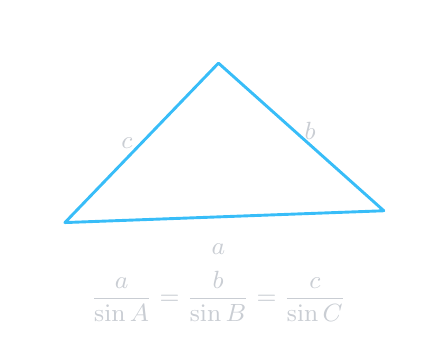
\begin{tikzpicture}[scale=0.75, line cap=round, line join=round, every node/.style={font=\small}]
  \coordinate (A) at (0,2.7);
  \coordinate (B) at (-2.6,0);
  \coordinate (C) at (2.8,0.2);
  \draw[strong] (A)--(B)--(C)--cycle;
  \node[lab] at (0,3.0) {$A$};
  \node[lab] at (-2.9,-0.2) {$B$};
  \node[lab] at (3.05,0.05) {$C$};
  \node[note] at (0,-0.45) {$a$};
  \node[note] at (1.55,1.55) {$b$};
  \node[note] at (-1.55,1.35) {$c$};
  \node[note] at (0,-1.25) {$\dfrac{a}{\sin A}=\dfrac{b}{\sin B}=\dfrac{c}{\sin C}$};
\end{tikzpicture}
\end{center}

% --- Law of Cosines diagram
\begin{center}
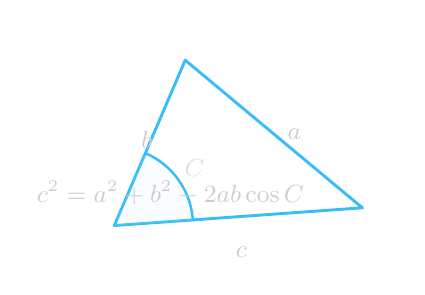
\begin{tikzpicture}[scale=0.75, line cap=round, line join=round, every node/.style={font=\small}]
  \coordinate (C) at (0,0);
  \coordinate (B) at (4.2,0.3);
  \coordinate (A) at (1.2,2.8);
  \draw[strong] (A)--(B)--(C)--cycle;
  \node[lab] at (1.2,3.05) {$A$};
  \node[lab] at (4.45,0.2) {$B$};
  \node[lab] at (-0.25,-0.1) {$C$};
  \node[note] at (2.15,-0.45) {$c$};
  \node[note] at (3.05,1.55) {$a$};
  \node[note] at (0.55,1.45) {$b$};
  \InternalAngle[IntAngle]{A}{C}{B}{C}
  \node[note] at (0.95,0.55) {$c^2=a^2+b^2-2ab\cos C$};
\end{tikzpicture}
\end{center}

% --- Area: 1/2 ab sin C diagram
\begin{center}
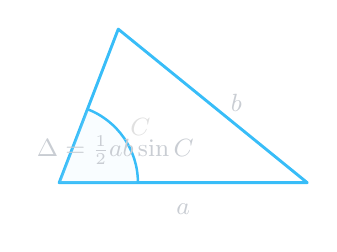
\begin{tikzpicture}[scale=0.75, line cap=round, line join=round, every node/.style={font=\small}]
  \coordinate (C) at (0,0);
  \coordinate (B) at (4.2,0);
  \coordinate (A) at (1.0,2.6);
  \draw[strong] (A)--(B)--(C)--cycle;
  \node[note] at (2.1,-0.45) {$a$};
  \node[note] at (3.0,1.35) {$b$};
  \InternalAngle[IntAngle]{B}{C}{A}{C}
  \node[note] at (0.95,0.55) {$\Delta=\frac12 ab\sin C$};
\end{tikzpicture}
\end{center}

% --- Right triangle: Pythagoras + trig ratio diagram
\begin{center}
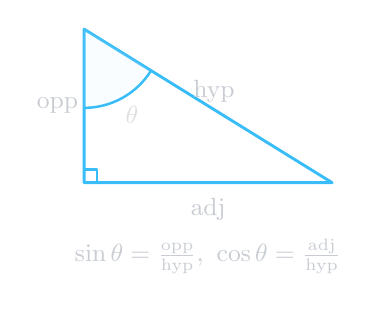
\begin{tikzpicture}[scale=0.75, line cap=round, line join=round, every node/.style={font=\small}]
  \coordinate (B) at (0,0);
  \coordinate (C) at (4.2,0);
  \coordinate (A) at (0,2.6);
  \draw[strong] (A)--(B)--(C)--cycle;
  \RightAngleMark{B}{0.22}
  \InternalAngle[IntAngle]{C}{A}{B}{\theta}
  \node[note] at (-0.45,1.3) {opp};
  \node[note] at (2.1,-0.45) {adj};
  \node[note] at (2.2,1.55) {hyp};
  \node[note] at (2.1,-1.25) {$\sin\theta=\frac{\text{opp}}{\text{hyp}},\ \cos\theta=\frac{\text{adj}}{\text{hyp}}$};
\end{tikzpicture}
\end{center}

% --- Chord in circle diagram
\begin{center}
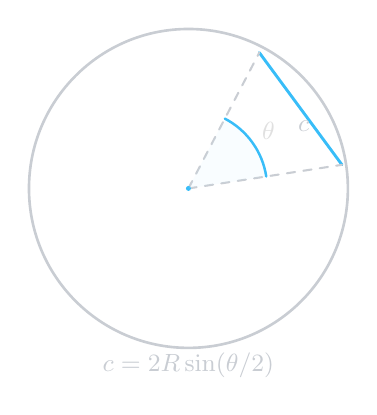
\begin{tikzpicture}[scale=0.75, line cap=round, line join=round, every node/.style={font=\small}]
  \coordinate (O) at (0,0);
  \coordinate (P) at (2.6,0.4);
  \coordinate (Q) at (1.2,2.3);
  \draw[geom] (O) circle(2.7);
  \draw[strong] (P)--(Q);
  \draw[helper] (O)--(P) (O)--(Q);
  \fill[pt] (O) circle(1.2pt) node[lab, below left] {$O$};
  \InternalAngle[IntAngle]{P}{O}{Q}{\theta}
  \node[note] at (1.95,1.05) {$c$};
  \node[note] at (0,-3.0) {$c=2R\sin(\theta/2)$};
\end{tikzpicture}
\end{center}

\end{QuickBox}

% ============================================================
% Q1 (MCQs)
\begin{QAPair}{Question 1 (i) --- MCQ}
\textcolor{gold}{\bfseries Question:} In right $\triangle ABC$, $a=2\text{ cm}$, $c=4\text{ cm}$, what is $\alpha$?\par
(a) $30^\circ$\quad (b) $45^\circ$\quad (c) $60^\circ$\quad (d) $120^\circ$
\tcblower
\textcolor{green}{\bfseries Answer:} \textbf{(a) $30^\circ$}\par

\Step{1} In a right triangle, if $c$ is the hypotenuse then $\sin\alpha=\dfrac{a}{c}=\dfrac{2}{4}=\dfrac12$.\par
\[
\Rightarrow \alpha=30^\circ.
\]

\StepFig{2}{Right triangle: $\sin\alpha=\frac{\text{opp}}{\text{hyp}}$.}{%
  \coordinate (B) at (0,0);
  \coordinate (C) at (4.2,0);
  \coordinate (A) at (0,2.6);
  \draw[strong] (A)--(B)--(C)--cycle;
  \RightAngleMark{B}{0.22}
  \node[lab] at (-0.25,1.3) {$a=2$};
  \node[lab] at (2.25,1.55) {$c=4$};
  \InternalAngle[IntAngle]{C}{A}{B}{}
  \node[lab] at (0.55,1.95) {$\alpha$};
}
\end{QAPair}

\begin{QAPair}{Question 1 (ii) --- MCQ}
\textcolor{gold}{\bfseries Question:} If in a triangle, $a=10$, $b=15$, $\alpha=32^\circ$, then $\beta=$\par
(a) $42.5^\circ$\quad (b) $46.5^\circ$\quad (c) $52.7^\circ$\quad (d) $62.8^\circ$
\tcblower
\textcolor{green}{\bfseries Answer:} \textbf{(c) $52.7^\circ$ (approx.)}\par

\Step{1} By Law of Sines:\quad $\displaystyle \frac{a}{\sin\alpha}=\frac{b}{\sin\beta}\Rightarrow \sin\beta=\frac{b\sin\alpha}{a}$.\par
\[
\sin\beta=\frac{15\sin 32^\circ}{10}=1.5\sin 32^\circ\approx 0.7949
\Rightarrow \beta\approx 52.7^\circ.
\]

\StepFig{2}{Law of sines picture (opposite sides).}{%
  \coordinate (A) at (0,2.4);
  \coordinate (B) at (-2.2,0);
  \coordinate (C) at (2.6,0.2);
  \draw[strong] (A)--(B)--(C)--cycle;
  \node[lab] at (0.0,2.65) {$A(\alpha)$};
  \node[lab] at (-2.45,-0.2) {$B(\beta)$};
  \node[lab] at (2.85,0.05) {$C$};
  \node[note] at (0.0,1.25) {$\dfrac{a}{\sin\alpha}=\dfrac{b}{\sin\beta}$};
}
\end{QAPair}

\begin{QAPair}{Question 1 (iii) --- MCQ}
\textcolor{gold}{\bfseries Question:} Area of an equilateral triangle having side $a$ is:\par
(a) $\dfrac{\sqrt3}{8}a$\quad
(b) $\dfrac{\sqrt3}{4}a^2$\quad
(c) $\dfrac{\sqrt3}{16}a^2$\quad
(d) $\cdots$
\tcblower
\textcolor{green}{\bfseries Answer:} \textbf{(b) $\dfrac{\sqrt3}{4}a^2$}\par

\Step{1} Height $h=\dfrac{\sqrt3}{2}a$, so\; $\Delta=\dfrac12 ah=\dfrac12 a\cdot \dfrac{\sqrt3}{2}a=\dfrac{\sqrt3}{4}a^2$.

\StepFig{2}{Equilateral triangle height split.}{%
  \coordinate (B) at (-2,0);
  \coordinate (C) at (2,0);
  \coordinate (A) at (0,3.0);
  \coordinate (M) at (0,0);
  \draw[strong] (A)--(B)--(C)--cycle;
  \draw[helper] (A)--(M);
  \RightAngleMark{M}{0.18}
  \node[lab] at (0,3.25) {$A$};
  \node[lab] at (-2.2,-0.2) {$B$};
  \node[lab] at (2.2,-0.2) {$C$};
  \node[note] at (1.1,1.4) {$h=\frac{\sqrt3}{2}a$};
  \node[note] at (0,-0.55) {base $=a$};
}
\end{QAPair}

\begin{QAPair}{Question 1 (iv) --- MCQ}
\textcolor{gold}{\bfseries Question:} If $a,a$ and $b$ are length sides of an isosceles triangle, then $S=$\ldots\par
(a) $\dfrac{a}{2}+b$ \quad
(b) $a+\dfrac{a+b}{2}$ \quad
(c) $a-\dfrac{a+b}{2}$ \quad
(d) $a+\dfrac{b}{2}$
\tcblower
\textcolor{green}{\bfseries Answer:} \textbf{(d) $S=a+\dfrac{b}{2}$}\par

\Step{1} Here $S$ means semiperimeter $s=\dfrac{a+a+b}{2}=a+\dfrac{b}{2}$.

\StepFig{2}{Isosceles sides $a,a$ and base $b$.}{%
  \coordinate (A) at (0,2.7);
  \coordinate (B) at (-2.2,0);
  \coordinate (C) at (2.2,0);
  \draw[strong] (A)--(B)--(C)--cycle;
  \node[note] at (-1.0,1.35) {$a$};
  \node[note] at (1.0,1.35) {$a$};
  \node[note] at (0,-0.35) {$b$};
  \node[draw=border, rounded corners=10pt, inner sep=8pt, text=text] at (0,-1.2)
  {$s=\dfrac{2a+b}{2}=a+\dfrac{b}{2}$};
}
\end{QAPair}

\begin{QAPair}{Question 1 (v) --- MCQ}
\textcolor{gold}{\bfseries Question:} Area of a triangle $ABC$ with $a=20$, $b=30$, $\gamma=90^\circ$ is:\par
(a) $0$\quad (b) $30$\quad (c) $300$\quad (d) $600$
\tcblower
\textcolor{green}{\bfseries Answer:} \textbf{(c) $300$}\par

\Step{1} Use $\Delta=\dfrac12 ab\sin\gamma$.\par
\[
\Delta=\frac12 (20)(30)\sin 90^\circ=\frac12\cdot 600\cdot 1=300.
\]

\StepFig{2}{Angle $\gamma$ between sides $a$ and $b$.}{%
  \coordinate (C) at (0,0);
  \coordinate (B) at (4.2,0);
  \coordinate (A) at (0,3.0);
  \draw[strong] (A)--(C)--(B)--cycle;
  \RightAngleMark{C}{0.22}
  \node[note] at (2.0,-0.35) {$b=30$};
  \node[note] at (-0.35,1.5) {$a=20$};
  \node[note] at (0.65,0.55) {$\gamma=90^\circ$};
}
\end{QAPair}

\begin{QAPair}{Question 1 (vi) --- MCQ}
\textcolor{gold}{\bfseries Question:} For an equilateral triangle, $r:r_1:R=$\ldots\par
(a) $1:2:3$\quad (b) $3:2:1$\quad (c) $1:1:2$\quad (d) $1:3:2$
\tcblower
\textcolor{green}{\bfseries Answer:} \textbf{(d) $1:3:2$}\par

\Step{1} For equilateral with side $a$:\;
$r=\dfrac{a\sqrt3}{6}$,\;
$R=\dfrac{a\sqrt3}{3}=2r$,\;
$r_1$ (an exradius) $=\dfrac{a\sqrt3}{2}=3r$.\par
So $r:r_1:R=1:3:2$.

\StepFig{2}{Same triangle: inradius smaller, exradius larger, circumradius medium.}{%
  \coordinate (B) at (-2,0);
  \coordinate (C) at (2,0);
  \coordinate (A) at (0,3.0);
  \coordinate (O) at (0,1.0);
  \draw[strong] (A)--(B)--(C)--cycle;
  \draw[geom] (O) circle(0.65);
  \draw[geom] (O) circle(1.30);
  \node[lab] at (0,1.0) {$O$};
  \node[note] at (0,-0.75) {$r<R<r_1$};
}
\end{QAPair}

\begin{QAPair}{Question 1 (vii) --- MCQ}
\textcolor{gold}{\bfseries Question:} Radius of circumcircle for sides $6,8,10$ is:\par
(a) $6$\quad (b) $5$\quad (c) $4$\quad (d) $2$
\tcblower
\textcolor{green}{\bfseries Answer:} \textbf{(b) $5$}\par

\Step{1} $6^2+8^2=10^2$ so it is a right triangle with hypotenuse $10$.\par
For a right triangle, circumradius $R=\dfrac{\text{hypotenuse}}{2}=\dfrac{10}{2}=5$.

\StepFig{2}{Right triangle in a circle: hypotenuse is the diameter.}{%
  \coordinate (B) at (-2.5,0);
  \coordinate (C) at (2.5,0);
  \coordinate (A) at (1.2,2.2);
  \coordinate (O) at (0,0);
  \draw[geom] (O) circle(2.5);
  \draw[strong] (A)--(B)--(C)--cycle;
  \draw[helper] (B)--(C);
  \node[note] at (0,-0.55) {Diameter $=10 \Rightarrow R=5$};
}
\end{QAPair}

\begin{QAPair}{Question 1 (viii) --- MCQ}
\textcolor{gold}{\bfseries Question:} If $a=5$, $b=10$, $c=20$ are sides of triangle $ABC$, then angle $\alpha$ is:\par
(a) not possible \quad (b) acute \quad (c) obtuse \quad (d) $0^\circ$
\tcblower
\textcolor{green}{\bfseries Answer:} \textbf{(a) not possible}\par

\Step{1} Triangle inequality must hold: $5+10>20$.\par
But $5+10=15<20$, so no triangle can be formed.

\StepFig{2}{Triangle inequality check.}{%
  \node[draw=cyan, rounded corners=12pt, inner sep=10pt, text=text] at (0,0.6)
  {$5+10<20\ \Rightarrow\ \text{No triangle}$};
  \draw[geom] (-2.2,-0.4) -- (2.2,-0.4);
  \node[note] at (0,-0.95) {Two short segments cannot reach the long one.};
}
\end{QAPair}

\begin{QAPair}{Question 1 (ix) --- MCQ}
\textcolor{gold}{\bfseries Question:} Radius of circum-circle $R=$\ldots\par
(a) $\dfrac{a}{2}\sec\!\dfrac{\alpha}{2}$\quad
(b) $\dfrac{b}{2}\sec\!\dfrac{\beta}{2}$\quad
(c) $\dfrac{c}{2}\csc\!\dfrac{\gamma}{2}$\quad
(d) $\dfrac{c}{2}\cos\!\dfrac{\gamma}{2}$
\tcblower
\textcolor{green}{\bfseries Answer:} \textbf{(c) $\dfrac{c}{2}\csc\!\left(\dfrac{\gamma}{2}\right)$}\par

\Step{1} Chord formula: if side $c$ is a chord subtending a \emph{central} angle $\gamma$, then\par
\[
c=2R\sin\left(\frac{\gamma}{2}\right)\ \Rightarrow\ 
R=\frac{c}{2\sin(\gamma/2)}=\frac{c}{2}\csc\left(\frac{\gamma}{2}\right).
\]

\StepFig{2}{Chord $c$ subtends central angle $\gamma$ (internal angle shown).}{%
  \coordinate (O) at (0,0);
  \coordinate (P) at (2.5,0.3);
  \coordinate (Q) at (1.1,2.2);
  \draw[geom] (O) circle(2.6);
  \draw[strong] (P)--(Q);
  \draw[helper] (O)--(P) (O)--(Q);
  \fill[pt] (O) circle(1.3pt) node[lab, below left] {$O$};
  \InternalAngle[IntAngle]{P}{O}{Q}{}
  \node[lab] at (0.75,0.55) {$\gamma$};
  \node[note] at (1.95,1.05) {$c$};
  \node[note] at (0,-3.0) {$c=2R\sin(\gamma/2)$};
}
\end{QAPair}

\begin{QAPair}{Question 1 (x) --- MCQ}
\textcolor{gold}{\bfseries Question:} If in a triangle $ABC$, $a=b=c$, then $\tan\left(\dfrac{\alpha}{2}\right)=$\ldots\par
(a) $\sqrt{\dfrac{s-a}{a}}$\quad
(b) $\sqrt{\dfrac{s-b}{b}}$\quad
(c) $\sqrt{\dfrac{s-c}{c}}$\quad
(d) all (a), (b) \& (c)
\tcblower
\textcolor{green}{\bfseries Answer:} \textbf{(d) all (a), (b) \& (c)}\par

\Step{1} If $a=b=c$, then $s=\dfrac{3a}{2}$ so $s-a=\dfrac{a}{2}$.\par
Each of (a),(b),(c) becomes $\sqrt{\dfrac{a/2}{a}}=\sqrt{\dfrac12}$, so all are the same.

\StepFig{2}{Equilateral case: symmetry makes all three forms equal.}{%
  \node[draw=cyan, rounded corners=12pt, inner sep=10pt, text=text] at (0,0.6)
  {$a=b=c\ \Rightarrow\ s-a=s-b=s-c=\dfrac{a}{2}$};
  \node[draw=border, rounded corners=12pt, inner sep=10pt, text=text] at (0,-0.55)
  {$\sqrt{\dfrac{s-a}{a}}=\sqrt{\dfrac{s-b}{b}}=\sqrt{\dfrac{s-c}{c}}=\sqrt{\dfrac12}$};
}
\end{QAPair}

\begin{QAPair}{Question 1 (xi) --- MCQ}
\textcolor{gold}{\bfseries Question:} Shadow of a man $5.6$ ft tall is making an angle of elevation of $45^\circ$ with the Sun. What is the length of shadow?\par
(a) $2.8$ ft \quad (b) $5.6$ ft \quad (c) $8.4$ ft \quad (d) $11.2$ ft
\tcblower
\textcolor{green}{\bfseries Answer:} \textbf{(b) $5.6$ ft}\par

\Step{1} In right triangle, $\tan 45^\circ=\dfrac{\text{height}}{\text{shadow}}=1$.\par
So shadow $=$ height $=5.6$ ft.

\StepFig{2}{Right triangle with $45^\circ$ (internal angle shown).}{%
  \coordinate (A) at (0,0);
  \coordinate (B) at (4.0,0);
  \coordinate (C) at (0,2.2);
  \draw[strong] (A)--(B)--(C)--cycle;
  \RightAngleMark{A}{0.20}
  \InternalAngle[IntAngle]{A}{B}{C}{}
  \node[lab] at (3.1,0.75) {$45^\circ$};
  \node[note] at (2.0,-0.35) {shadow};
  \node[note] at (-0.55,1.1) {height};
}
\end{QAPair}

\begin{QAPair}{Question 1 (xii) --- MCQ}
\textcolor{gold}{\bfseries Question:} $R(\sin\alpha+\sin\beta+\sin\gamma)=$\ldots\par
(a) $S$\quad (b) $S^2$\quad (c) $\dfrac{1}{S}$\quad (d) $\dfrac{1}{S^2}$
\tcblower
\textcolor{green}{\bfseries Answer:} \textbf{(a) $S$ (i.e., semiperimeter $s$)}\par

\Step{1} From Law of Sines: $a=2R\sin\alpha$, $b=2R\sin\beta$, $c=2R\sin\gamma$.\par
Add:
\[
a+b+c=2R(\sin\alpha+\sin\beta+\sin\gamma)
\]
Divide by $2$:
\[
\frac{a+b+c}{2}=R(\sin\alpha+\sin\beta+\sin\gamma)=s=S.
\]

\StepFig{2}{Extended sine rule idea.}{%
  \node[draw=border, rounded corners=12pt, inner sep=10pt, text=text] at (0,0.6)
  {$a=2R\sin\alpha,\ b=2R\sin\beta,\ c=2R\sin\gamma$};
  \node[draw=cyan, rounded corners=12pt, inner sep=10pt, text=text] at (0,-0.55)
  {$R(\sin\alpha+\sin\beta+\sin\gamma)=\dfrac{a+b+c}{2}=s$};
}
\end{QAPair}

% ============================================================
% Q2 Oblique triangles
\begin{QAPair}{Question 2 --- Solve the following oblique triangles}
\textcolor{gold}{\bfseries (i) $a=8,\ \alpha=15^\circ,\ \beta=20^\circ$}\par
\Step{1} $\gamma=180^\circ-15^\circ-20^\circ=145^\circ$.\par
\Step{2} Law of sines:
\[
\frac{a}{\sin\alpha}=\frac{b}{\sin\beta}=\frac{c}{\sin\gamma}
\Rightarrow
b\approx 10.57,\quad c\approx 17.73.
\]

\StepFig{3}{Triangle sketch (angles shown).}{%
  \coordinate (A) at (0,2.6);
  \coordinate (B) at (-2.4,0);
  \coordinate (C) at (2.6,0.2);
  \draw[strong] (A)--(B)--(C)--cycle;
  \node[lab] at (0,2.85) {$\alpha=15^\circ$};
  \node[lab] at (-2.7,-0.2) {$\beta=20^\circ$};
  \node[lab] at (2.85,0.05) {$\gamma=145^\circ$};
}

\textcolor{gold}{\bfseries Answer (i):}\quad
$\boxed{\gamma=145^\circ,\ b\approx 10.6,\ c\approx 17.7}$\par\medskip

\textcolor{gold}{\bfseries (ii) $a=34,\ b=41,\ \alpha=115^\circ$}\par
\Step{1} Since $\alpha$ is obtuse, side $a$ must be the \emph{largest} side.\par
But $b=41>a=34$, so this is impossible.\par
(Equivalently, by Law of Sines: $\sin\beta=\dfrac{b\sin\alpha}{a}=\dfrac{41\sin115^\circ}{34}>1$.)

\StepFig{2}{Why impossible (largest angle needs largest opposite side).}{%
  \node[draw=cyan, rounded corners=12pt, inner sep=10pt, text=text] at (0,0.65)
  {$\alpha=115^\circ\ \text{is largest} \Rightarrow a\ \text{must be largest}$};
  \node[draw=border, rounded corners=12pt, inner sep=10pt, text=text] at (0,-0.55)
  {$\text{But } b=41>a=34\ \Rightarrow\ \text{No triangle.}$};
}

\textcolor{gold}{\bfseries Answer (ii):}\quad
$\boxed{\text{No solution (triangle not possible).}}$\par\medskip

\textcolor{gold}{\bfseries (iii) $b=17.3,\ c=14.5,\ \beta=98.2^\circ$}\par
\Step{1} Law of sines:\ $\sin\gamma=\dfrac{c\sin\beta}{b}\Rightarrow \gamma\approx 56.1^\circ$.\par
\Step{2} $\alpha=180^\circ-\beta-\gamma\approx 25.7^\circ$.\par
\Step{3} $a=\dfrac{b\sin\alpha}{\sin\beta}\approx 7.59$.

\StepFig{3}{Oblique triangle (one obtuse angle).}{%
  \coordinate (B) at (-2.6,0);
  \coordinate (C) at (2.5,0.2);
  \coordinate (A) at (-0.2,2.8);
  \draw[strong] (A)--(B)--(C)--cycle;
  \node[lab] at (-2.95,-0.2) {$\beta=98.2^\circ$};
  \node[lab] at (2.8,0.05) {$\gamma\approx 56.1^\circ$};
  \node[lab] at (-0.2,3.05) {$\alpha\approx 25.7^\circ$};
}

\textcolor{gold}{\bfseries Answer (iii):}\quad
$\boxed{\alpha\approx 25.7^\circ,\ \gamma\approx 56.1^\circ,\ a\approx 7.6}$\par\medskip

\textcolor{gold}{\bfseries (iv) $c=65.4,\ \alpha=115^\circ,\ \beta=45^\circ$}\par
\Step{1} $\gamma=180^\circ-115^\circ-45^\circ=20^\circ$.\par
\Step{2} Law of sines:
\[
a=\frac{c\sin\alpha}{\sin\gamma}\approx 173.31,\qquad
b=\frac{c\sin\beta}{\sin\gamma}\approx 135.19.
\]

\StepFig{3}{Small $\gamma$ makes the opposite side large.}{%
  \coordinate (A) at (-0.4,2.8);
  \coordinate (B) at (-2.8,0);
  \coordinate (C) at (2.8,0.15);
  \draw[strong] (A)--(B)--(C)--cycle;
  \node[lab] at (-0.4,3.05) {$\alpha=115^\circ$};
  \node[lab] at (-3.15,-0.2) {$\beta=45^\circ$};
  \node[lab] at (2.95,0.05) {$\gamma=20^\circ$};
}

\textcolor{gold}{\bfseries Answer (iv):}\quad
$\boxed{\gamma=20^\circ,\ a\approx 173.3,\ b\approx 135.2}$\par\medskip

\textcolor{gold}{\bfseries (v) $a=34,\ c=48,\ \beta=108^\circ$}\par
\Step{1} Use cosine rule for side $b$ (opposite $\beta$):
\[
b^2=a^2+c^2-2ac\cos\beta \ \Rightarrow\ b\approx 66.97.
\]
\Step{2} Law of sines:
\[
\sin\alpha=\frac{a\sin\beta}{b}\Rightarrow \alpha\approx 25.4^\circ,\quad
\gamma=180^\circ-\alpha-\beta\approx 46.6^\circ.
\]

\StepFig{3}{SAS setup: $a$ and $c$ around $\beta$.}{%
  \coordinate (B) at (0,0);
  \coordinate (A) at (-2.6,0.2);
  \coordinate (C) at (1.0,2.8);
  \draw[strong] (A)--(B)--(C)--cycle;
  \node[lab] at (0.25,0.55) {$\beta=108^\circ$};
  \node[note] at (-1.1,0.25) {$c=48$};
  \node[note] at (0.65,1.45) {$a=34$};
}

\textcolor{gold}{\bfseries Answer (v):}\quad
$\boxed{b\approx 67.0,\ \alpha\approx 25.4^\circ,\ \gamma\approx 46.6^\circ}$\par\medskip

\textcolor{gold}{\bfseries (vi) $a=44,\ b=33,\ c=55$}\par
\Step{1} Cosine rule:
\[
\cos C=\frac{a^2+b^2-c^2}{2ab}\Rightarrow C=90^\circ.
\]
\Step{2} Then
\[
A\approx 52.9^\circ,\qquad B\approx 37.1^\circ.
\]

\StepFig{3}{This one turns out to be right-angled ($C=90^\circ$).}{%
  \coordinate (C) at (0,0);
  \coordinate (B) at (4.2,0);
  \coordinate (A) at (0,3.0);
  \draw[strong] (A)--(C)--(B)--cycle;
  \RightAngleMark{C}{0.22}
  \node[note] at (2.0,-0.35) {$a=44$};
  \node[note] at (-0.35,1.5) {$b=33$};
  \node[note] at (2.2,1.55) {$c=55$};
}

\textcolor{gold}{\bfseries Answer (vi):}\quad
$\boxed{A\approx 52.9^\circ,\ B\approx 37.1^\circ,\ C=90^\circ}$
\end{QAPair}

% ============================================================
% Q3
\begin{QAPair}{Question 3 --- Parallelogram diagonals}
\textcolor{gold}{\bfseries Question:} The diagonals of a parallelogram measure $12$ cm and $22$ cm and intersect at an angle of $143^\circ$. Find the length of the longer sides of the parallelogram.\par

\textcolor{gold}{\bfseries Working:}\par
Let diagonals be vectors $\vec d_1,\vec d_2$ with $|\vec d_1|=12$, $|\vec d_2|=22$, and angle between them $\theta=143^\circ$.
The side vectors are
\[
\vec u=\frac{\vec d_1+\vec d_2}{2},\qquad
\vec v=\frac{\vec d_1-\vec d_2}{2}.
\]
So
\[
|\vec u|^2=\frac{12^2+22^2+2(12)(22)\cos\theta}{4},\quad
|\vec v|^2=\frac{12^2+22^2-2(12)(22)\cos\theta}{4}.
\]
Since $\cos 143^\circ<0$, the \textbf{longer} side is $|\vec v|$.
\[
|\vec v|\approx 16.20\text{ cm}.
\]

\StepFig{2}{Diagonals crossing (internal angle shown).}{%
  \coordinate (O) at (0,0);
  \coordinate (P) at (-2.8,-0.6);
  \coordinate (Q) at (2.8,0.6);
  \coordinate (R) at (-1.2,2.3);
  \coordinate (S) at (1.2,-2.3);
  \draw[strong] (R)--(Q)--(S)--(P)--cycle; % rough parallelogram look
  \draw[geom] (R)--(S);
  \draw[geom] (P)--(Q);
  \InternalAngle[IntAngle]{R}{O}{P}{}
  \node[lab] at (-0.7,0.55) {$143^\circ$};
  \fill[pt] (O) circle(1.3pt);
  \node[note] at (0,-2.9) {Longer side uses $12^2+22^2-2(12)(22)\cos 143^\circ$};
}

\tcblower
\textcolor{green}{\bfseries Answer:}\quad $\boxed{16.20\text{ cm (approx.)}}$
\end{QAPair}

% ============================================================
% Q4
\begin{QAPair}{Question 4 --- Triangular walk}
\textcolor{gold}{\bfseries Question:} Walk $1.5$ km, turn at angle $100^\circ$, walk $0.95$ km, then return home.\par
(a) Find the last portion.\qquad (b) Find total distance.\par

\textcolor{gold}{\bfseries Working:}\par
Let the two walked sides be $1.5$ and $0.95$ with included angle $100^\circ$. Return distance $x$ is opposite $100^\circ$.
\[
x^2=1.5^2+0.95^2-2(1.5)(0.95)\cos 100^\circ
\Rightarrow x\approx 1.91\text{ km}.
\]
Total distance:
\[
1.5+0.95+1.91\approx 4.36\text{ km}.
\]

\StepFig{2}{Triangle path diagram (internal angle shown).}{%
  \coordinate (H) at (0,0);
  \coordinate (T) at (4.0,0);
  \coordinate (U) at (2.1,2.3);
  \draw[strong] (H)--(T)--(U)--cycle;
  \node[note] at (2.0,-0.35) {$1.5$ km};
  \node[note] at (3.35,1.25) {$0.95$ km};
  \node[note] at (1.0,1.25) {$x$};
  \InternalAngle[IntAngle]{H}{T}{U}{}
  \node[lab] at (3.15,0.55) {$100^\circ$};
}

\tcblower
\textcolor{green}{\bfseries Answers:}\par
(a) $\boxed{x\approx 1.91\text{ km}}$\par
(b) $\boxed{\text{Total}\approx 4.36\text{ km}}$
\end{QAPair}

% ============================================================
% Q5
\begin{QAPair}{Question 5 --- Kite (two pairs of equal adjacent sides)}
\textcolor{gold}{\bfseries Question:} A kite has sides $20,20,35,35$ inches. The two shorter sides meet at $115^\circ$.\par
(a) Find the diagonal between the points where the unequal sides meet.\par
(b) Using (a), find the angle at which the longer sides meet.\par

\textcolor{gold}{\bfseries Working:}\par
Let $AB=AD=20$ meet at $A$ with $\angle BAD=115^\circ$. Then diagonal $BD$ is opposite $115^\circ$ in $\triangle ABD$:
\[
BD^2=20^2+20^2-2(20)(20)\cos 115^\circ\Rightarrow BD\approx 36.28\text{ in}.
\]
Now in $\triangle BCD$ with $BC=CD=35$ and base $BD$:
\[
\cos\angle BCD=\frac{35^2+35^2-BD^2}{2(35)(35)}
\Rightarrow \angle BCD\approx 57.6^\circ.
\]

\StepFig{2}{Kite sketch and diagonal $BD$ (internal angle shown).}{%
  \coordinate (A) at (0,2.6);
  \coordinate (B) at (-2.4,0);
  \coordinate (D) at (2.4,0);
  \coordinate (C) at (0,-2.2);
  \draw[strong] (A)--(B)--(C)--(D)--cycle;
  \draw[geom] (B)--(D);
  \node[note] at (-1.3,1.35) {$20$};
  \node[note] at (1.3,1.35) {$20$};
  \node[note] at (-1.3,-1.3) {$35$};
  \node[note] at (1.3,-1.3) {$35$};
  \InternalAngle[IntAngle]{B}{A}{D}{}
  \node[lab] at (0.25,2.0) {$115^\circ$};
  \node[note] at (0,0.35) {$BD$};
}

\tcblower
\textcolor{green}{\bfseries Answers:}\par
(a) $\boxed{BD\approx 36.28\text{ in}}$\par
(b) $\boxed{\angle(\text{longer sides})\approx 57.6^\circ}$
\end{QAPair}

% ============================================================
% Q6
\begin{QAPair}{Question 6 --- Area of park (Heron's formula)}
\textcolor{gold}{\bfseries Question:} Three streets enclose a triangular park with sides $55$ m, $63$ m, and $77$ m. Find its area.\par

\textcolor{gold}{\bfseries Working:}\par
\[
s=\frac{55+63+77}{2}=97.5
\]
\[
\Delta=\sqrt{s(s-a)(s-b)(s-c)}
=\sqrt{97.5(42.5)(34.5)(20.5)}
\approx 1711.92\ \text{m}^2.
\]

\StepFig{2}{Triangle with three given sides.}{%
  \coordinate (A) at (0,2.6);
  \coordinate (B) at (-2.6,0);
  \coordinate (C) at (2.8,0.2);
  \draw[strong] (A)--(B)--(C)--cycle;
  \node[note] at (-1.3,1.3) {$55$};
  \node[note] at (1.5,1.35) {$63$};
  \node[note] at (0,-0.35) {$77$};
  \node[note] at (0,-1.1) {Use Heron's formula};
}

\tcblower
\textcolor{green}{\bfseries Answer:}\quad $\boxed{\Delta\approx 1711.9\ \text{m}^2}$
\end{QAPair}

% ============================================================
% Q7
\begin{QAPair}{Question 7 --- Isosceles triangle (base and vertex angle)}
\textcolor{gold}{\bfseries Question:} The base of an isosceles triangle is $14.5$ cm and the vertex angle is $110^\circ$.\par
(a) Find one congruent side.\qquad (b) Find perimeter.\par

\textcolor{gold}{\bfseries Working:}\par
Let equal sides be $x,x$ and base be $14.5$, opposite vertex angle $110^\circ$.
\[
14.5^2=x^2+x^2-2x^2\cos110^\circ
=2x^2(1-\cos110^\circ)
\Rightarrow x\approx 8.85\text{ cm}.
\]
Perimeter:
\[
P=2x+14.5\approx 2(8.85)+14.5\approx 32.20\text{ cm}.
\]

\StepFig{2}{Isosceles triangle with vertex angle $110^\circ$ (internal angle shown).}{%
  \coordinate (A) at (0,2.7);
  \coordinate (B) at (-2.6,0);
  \coordinate (C) at (2.6,0);
  \draw[strong] (A)--(B)--(C)--cycle;
  \InternalAngle[IntAngle]{B}{A}{C}{}
  \node[lab] at (0.25,2.05) {$110^\circ$};
  \node[note] at (0,-0.35) {$14.5$};
  \node[note] at (-1.2,1.35) {$x$};
  \node[note] at (1.2,1.35) {$x$};
}

\tcblower
\textcolor{green}{\bfseries Answers:}\par
(a) $\boxed{x\approx 8.85\text{ cm}}$\par
(b) $\boxed{P\approx 32.20\text{ cm}}$
\end{QAPair}

% ============================================================
% Q8
\begin{QAPair}{Question 8 --- Triangle from angles and longest side}
\textcolor{gold}{\bfseries Question:} Two angles are $80^\circ$ and $60^\circ$. The longest side is $90$ m. Find the other two sides.\par

\textcolor{gold}{\bfseries Working:}\par
Third angle $=180^\circ-80^\circ-60^\circ=40^\circ$.\par
Largest angle is $80^\circ$, so the side opposite it is the longest: let $a=90$ opposite $80^\circ$.\par
By Law of Sines:
\[
b=\frac{a\sin 60^\circ}{\sin 80^\circ}\approx 79.14\text{ m},\qquad
c=\frac{a\sin 40^\circ}{\sin 80^\circ}\approx 58.74\text{ m}.
\]

\StepFig{2}{Angle-side correspondence (largest angle opposite longest side).}{%
  \coordinate (A) at (0,2.8);
  \coordinate (B) at (-2.8,0);
  \coordinate (C) at (2.8,0.1);
  \draw[strong] (A)--(B)--(C)--cycle;
  \node[lab] at (0,3.05) {$80^\circ$};
  \node[lab] at (-3.1,-0.2) {$60^\circ$};
  \node[lab] at (3.05,0.0) {$40^\circ$};
  \node[note] at (0,-0.35) {opposite $80^\circ$: $90$m};
}

\tcblower
\textcolor{green}{\bfseries Answer:}\quad $\boxed{79.14\text{ m and }58.74\text{ m (approx.)}}$
\end{QAPair}

% ============================================================
% Q9
\begin{QAPair}{Question 9 --- Parallelogram possibility}
\textcolor{gold}{\bfseries Question:} Aamir wants to draw a parallelogram with one side $12$ cm, one diagonal $10$ cm and one angle $120^\circ$. Is this possible? Explain (Hint: Law of Sines).\par

\tcblower
\textcolor{green}{\bfseries Answer:} \textbf{Not possible.}\par
Consider the triangle formed by the side $12$ cm and the diagonal $10$ cm with included angle $120^\circ$ at the vertex.
In any triangle, the side opposite the \textbf{largest angle} must be the \textbf{largest side}. But $120^\circ$ is obtuse (largest), so the opposite side should be longer than $12$ cm; however the diagonal is $10$ cm.\par
Also by Law of Sines (taking diagonal opposite $120^\circ$):
\[
\frac{10}{\sin120^\circ}=\frac{12}{\sin\theta}
\Rightarrow \sin\theta=\frac{12\sin120^\circ}{10}>1,
\]
which is impossible. Hence no such parallelogram can be drawn.

\StepFig{1}{Sine-law contradiction ($\sin\theta>1$).}{%
  \node[draw=cyan, rounded corners=12pt, inner sep=10pt, text=text] at (0,0.6)
  {$\sin\theta=\dfrac{12\sin120^\circ}{10}>1\ \Rightarrow\ \text{impossible}$};
  \node[note] at (0,-0.55) {So the given measurements cannot form the needed triangle.};
}
\end{QAPair}

% ============================================================
% Q10
\begin{QAPair}{Question 10 --- Depression / inclination to a pipe}
\textcolor{gold}{\bfseries Question:} Angle of depression from an observer to a pipe is $55^\circ$. From a point five stories below, the angle of inclination to the pipe is $20^\circ$. One story is $9$ ft.\par
Find:\par
(i) distance from each observer to the pipe,\quad
(ii) distance between the pipe and the apartment complex.\par

\textcolor{gold}{\bfseries Working:}\par
Vertical separation between observers $=5\times 9=45$ ft.\par
Let horizontal distance between buildings be $x$.\par
From top observer: $\tan55^\circ=\dfrac{\text{drop}}{x}$.\par
From lower observer: $\tan20^\circ=\dfrac{\text{rise}}{x}$.\par
But drop + rise $=45$, so
\[
45=x(\tan55^\circ+\tan20^\circ)
\Rightarrow x=\frac{45}{\tan55^\circ+\tan20^\circ}\approx 25.11\text{ ft}.
\]
Distances to the pipe (hypotenuse):
\[
d_1=\frac{x}{\cos55^\circ}\approx 43.78\text{ ft},\qquad
d_2=\frac{x}{\cos20^\circ}\approx 26.72\text{ ft}.
\]

\StepFig{2}{Two observers (left) and pipe (right).}{%
  \coordinate (O2) at (0,0);
  \coordinate (O1) at (0,3.6);
  \coordinate (P) at (4.2,1.0);
  \draw[geom] (0,-0.2)--(0,4.1); % building
  \draw[geom] (4.2,-0.2)--(4.2,3.3); % other building
  \draw[strong] (O1)--(P);
  \draw[strong] (O2)--(P);
  \draw[helper] (O1)--(4.2,3.6);
  \draw[helper] (O2)--(4.2,0);
  \node[lab] at (-0.4,3.6) {Top};
  \node[lab] at (-0.55,0.0) {Lower};
  \node[lab] at (4.55,1.0) {Pipe};
  \node[note] at (2.1,3.0) {$55^\circ$};
  \node[note] at (2.1,0.55) {$20^\circ$};
  \node[note] at (-0.9,1.8) {$45$ ft};
  \node[note] at (2.1,-0.55) {$x$};
}

\tcblower
\textcolor{green}{\bfseries Answers:}\par
Distance building-to-building: $\boxed{x\approx 25.11\text{ ft}}$\par
Top observer to pipe: $\boxed{d_1\approx 43.78\text{ ft}}$\par
Lower observer to pipe: $\boxed{d_2\approx 26.72\text{ ft}}$
\end{QAPair}

% ============================================================
% Q11
\begin{QAPair}{Question 11 --- Crater diameter}
\textcolor{gold}{\bfseries Question:} From camp, distance to northern-most point is $4$ miles and to southern-most point is $2$ miles. Angle between lines of sight is $117^\circ$. Find the crater diameter.\par

\textcolor{gold}{\bfseries Working:}\par
This is a triangle with sides $4$ and $2$ including angle $117^\circ$. Diameter is the side opposite $117^\circ$:
\[
d^2=4^2+2^2-2(4)(2)\cos117^\circ
\Rightarrow d\approx 5.22\text{ miles}.
\]

\StepFig{2}{Camp and two sight lines (internal angle shown).}{%
  \coordinate (C) at (0,0);
  \coordinate (N) at (4.0,0.3);
  \coordinate (S) at (1.2,3.3);
  \draw[strong] (C)--(N);
  \draw[strong] (C)--(S);
  \draw[geom] (N)--(S);
  \InternalAngle[IntAngle]{N}{C}{S}{}
  \node[lab] at (0.65,0.95) {$117^\circ$};
  \node[note] at (2.0,0.15) {$4$};
  \node[note] at (0.55,1.9) {$2$};
  \node[note] at (2.25,2.05) {diameter $d$};
}
\tcblower
\textcolor{green}{\bfseries Answer:}\quad $\boxed{d\approx 5.22\text{ miles}}$
\end{QAPair}

% ============================================================
% Q12
\begin{QAPair}{Question 12 --- Circumference of circumcircle and excircle (equilateral)}
\textcolor{gold}{\bfseries Question:} Side of an equilateral triangle is $6$ cm. Find the circumference of circumcircle and ex-circle.\par

\textcolor{gold}{\bfseries Working:}\par
For equilateral, $R=\dfrac{a}{\sqrt3}$ and exradius $r_a=\dfrac{a\sqrt3}{2}$.
With $a=6$:
\[
R=\frac{6}{\sqrt3}=2\sqrt3,\qquad r_a=\frac{6\sqrt3}{2}=3\sqrt3.
\]
Circumferences:
\[
C_{\text{circ}}=2\pi R=2\pi(2\sqrt3)=4\pi\sqrt3\ \text{cm},
\]
\[
C_{\text{ex}}=2\pi r_a=2\pi(3\sqrt3)=6\pi\sqrt3\ \text{cm}.
\]

\StepFig{2}{Equilateral triangle with circumcircle.}{%
  \coordinate (B) at (-2,0);
  \coordinate (C) at (2,0);
  \coordinate (A) at (0,3.0);
  \coordinate (O) at (0,1.0);
  \draw[strong] (A)--(B)--(C)--cycle;
  \draw[geom] (O) circle(1.35);
  \fill[pt] (O) circle(1.2pt) node[lab, left] {$O$};
  \node[note] at (0,-0.65) {$a=6$};
}

\tcblower
\textcolor{green}{\bfseries Answers:}\par
$\boxed{C_{\text{circ}}=4\pi\sqrt3\ \text{cm}\ (\approx 21.77\text{ cm})}$\par
$\boxed{C_{\text{ex}}=6\pi\sqrt3\ \text{cm}\ (\approx 32.65\text{ cm})}$
\end{QAPair}

% ============================================================
% Q13
\begin{QAPair}{Question 13 --- Prove triangle is equilateral (Law of Cosines)}
\textcolor{gold}{\bfseries Question:} Use the Law of Cosines to prove that if the angle between two congruent sides of a triangle is $60^\circ$, the triangle is equilateral.\par

\tcblower
\textcolor{green}{\bfseries Proof:}\par
Let $AB=AC=a$ and $\angle A=60^\circ$. By Law of Cosines on side $BC$:
\[
BC^2=AB^2+AC^2-2(AB)(AC)\cos A
=a^2+a^2-2a^2\cos 60^\circ
=2a^2-2a^2\cdot \frac12
=a^2.
\]
So $BC=a$. Hence $AB=AC=BC$, therefore the triangle is \textbf{equilateral}.

\StepFig{1}{Two equal sides with included $60^\circ$ (internal angle shown).}{%
  \coordinate (A) at (0,2.7);
  \coordinate (B) at (-2.4,0);
  \coordinate (C) at (2.4,0);
  \draw[strong] (A)--(B)--(C)--cycle;
  \InternalAngle[IntAngle]{B}{A}{C}{}
  \node[lab] at (0.25,2.05) {$60^\circ$};
  \node[note] at (-1.2,1.35) {$a$};
  \node[note] at (1.2,1.35) {$a$};
}
\end{QAPair}

% ============================================================
% Q14
\begin{QAPair}{Question 14 --- Prove an identity with $r,r_1,r_2,r_3$}
\textcolor{gold}{\bfseries Statement:}\quad
\[
\frac{1}{r^2}+\frac{1}{r_1^2}+\frac{1}{r_2^2}+\frac{1}{r_3^2}
=\frac{a^2+b^2+c^2}{\Delta^2}.
\]
(Here $r$ is inradius, $r_1,r_2,r_3$ are the three exradii, and $\Delta$ is the area.)\par

\tcblower
\textcolor{green}{\bfseries Proof:}\par
Recall
\[
r=\frac{\Delta}{s},\qquad r_1=\frac{\Delta}{s-a},\qquad r_2=\frac{\Delta}{s-b},\qquad r_3=\frac{\Delta}{s-c}.
\]
So
\[
\frac{1}{r^2}=\frac{s^2}{\Delta^2},\qquad
\frac{1}{r_1^2}=\frac{(s-a)^2}{\Delta^2},\qquad \text{etc.}
\]
Hence
\[
\frac{1}{r^2}+\frac{1}{r_1^2}+\frac{1}{r_2^2}+\frac{1}{r_3^2}
=\frac{s^2+(s-a)^2+(s-b)^2+(s-c)^2}{\Delta^2}.
\]
Now expand the numerator:
\[
s^2+(s-a)^2+(s-b)^2+(s-c)^2
=4s^2-2s(a+b+c)+(a^2+b^2+c^2).
\]
But $a+b+c=2s$, so
\[
4s^2-2s(2s)+(a^2+b^2+c^2)=a^2+b^2+c^2.
\]
Therefore
\[
\frac{1}{r^2}+\frac{1}{r_1^2}+\frac{1}{r_2^2}+\frac{1}{r_3^2}
=\frac{a^2+b^2+c^2}{\Delta^2}.
\]
\end{QAPair}

% ============================================================
% Q15
\begin{QAPair}{Question 15 --- Prove exradius half-angle formulas}
\textcolor{gold}{\bfseries Statement:}\par
\[
\text{(i)}\ \ r_1=a\cos\frac{\beta}{2}\cos\frac{\gamma}{2}\sec\frac{\alpha}{2},\qquad
\text{(ii)}\ \ r_2=b\cos\frac{\alpha}{2}\cos\frac{\gamma}{2}\sec\frac{\beta}{2},
\]
\[
\text{(iii)}\ \ r_3=c\cos\frac{\alpha}{2}\cos\frac{\beta}{2}\sec\frac{\gamma}{2}.
\]

\tcblower
\textcolor{green}{\bfseries Proof (same method for all):}\par
A known half-angle formula for the $A$-exradius is
\[
r_1=r_a=4R\sin\frac{\alpha}{2}\cos\frac{\beta}{2}\cos\frac{\gamma}{2}.
\]
Also, from extended Law of Sines: $a=2R\sin\alpha$ and $\sin\alpha=2\sin\frac{\alpha}{2}\cos\frac{\alpha}{2}$, so
\[
a=2R\cdot 2\sin\frac{\alpha}{2}\cos\frac{\alpha}{2}
=4R\sin\frac{\alpha}{2}\cos\frac{\alpha}{2}.
\]
Therefore
\[
r_1=4R\sin\frac{\alpha}{2}\cos\frac{\beta}{2}\cos\frac{\gamma}{2}
=\Big(4R\sin\frac{\alpha}{2}\cos\frac{\alpha}{2}\Big)\,
\cos\frac{\beta}{2}\cos\frac{\gamma}{2}\sec\frac{\alpha}{2}
\]
\[
= a\cos\frac{\beta}{2}\cos\frac{\gamma}{2}\sec\frac{\alpha}{2}.
\]
Similarly, cyclic replacement $(a,\alpha)\to(b,\beta)\to(c,\gamma)$ gives (ii) and (iii).
\end{QAPair}

% ============================================================
% Q16
\begin{QAPair}{Question 16 --- Mountain tunnel length}
\textcolor{gold}{\bfseries Question:} A mountain climber is on top of a mountain $680$ m high. Angles of depression to two points on opposite sides are $48^\circ$ and $32^\circ$. How long would a tunnel between the points be?\par

\textcolor{gold}{\bfseries Working:}\par
If height is $h$, and angle of depression is $\theta$, horizontal distance is $d=\dfrac{h}{\tan\theta}$.\par
So
\[
d_1=\frac{680}{\tan48^\circ}\approx 612.64\text{ m},\qquad
d_2=\frac{680}{\tan32^\circ}\approx 1087.87\text{ m}.
\]
Points are on opposite sides, so tunnel length
\[
L=d_1+d_2\approx 1700.50\text{ m}.
\]

\StepFig{2}{Two right triangles back-to-back.}{%
  \coordinate (T) at (0,2.8);
  \coordinate (B) at (0,0);
  \coordinate (P1) at (-3.2,0);
  \coordinate (P2) at (4.4,0);
  \draw[geom] (P1)--(P2);
  \draw[strong] (T)--(P1);
  \draw[strong] (T)--(P2);
  \draw[helper] (T)--(0,0);
  \node[note] at (0.3,1.4) {$680$ m};
  \node[note] at (-1.6,1.25) {$48^\circ$};
  \node[note] at (2.4,1.25) {$32^\circ$};
  \node[note] at (0,-0.55) {$L=d_1+d_2$};
}

\tcblower
\textcolor{green}{\bfseries Answer:}\quad $\boxed{L\approx 1700.5\text{ m}}$
\end{QAPair}

% ============================================================
% Q17
\begin{QAPair}{Question 17 --- Find $\angle C$ in the figure}
\textcolor{gold}{\bfseries Given (from figure):} $AD=12.6$ cm, $\angle A=37^\circ$, $DC=22.5$ cm, and $BD\perp AD$, $BD\perp BC$.\par

\textcolor{gold}{\bfseries Working:}\par
In right $\triangle ABD$:
\[
BD=AD\tan 37^\circ=12.6\tan37^\circ\approx 9.49\text{ cm}.
\]
In right $\triangle BDC$ (right at $B$), with hypotenuse $DC=22.5$:
\[
\sin\angle C=\frac{BD}{DC}\approx \frac{9.49}{22.5}
\Rightarrow \angle C\approx 25.0^\circ.
\]

\StepFig{2}{Re-draw as two right triangles (internal angle shown).}{%
  \coordinate (A) at (0,0);
  \coordinate (D) at (4.2,0);
  \coordinate (B) at (4.2,2.3);
  \coordinate (C) at (7.2,2.3);
  \draw[strong] (A)--(D)--(B)--(C);
  \draw[strong] (D)--(C);
  \RightAngleMark{D}{0.18}
  \RightAngleMark{B}{0.18}
  \InternalAngle[IntAngle]{D}{A}{B}{}
  \node[lab] at (0.75,0.55) {$37^\circ$};
  \node[note] at (2.1,-0.35) {$12.6$};
  \node[note] at (5.8,1.1) {$22.5$};
}

\tcblower
\textcolor{green}{\bfseries Answer:}\quad $\boxed{\angle C\approx 25.0^\circ}$
\end{QAPair}

% ============================================================
% Q18
\begin{QAPair}{Question 18 --- Square prism (find angle $a$)}
\textcolor{gold}{\bfseries Question:} Sides of a square prism are $12$ cm, $5$ cm and $5$ cm as shown. Find angle $a$.\par

\textcolor{gold}{\bfseries Interpretation:} $a$ is angle between the base diagonal $AC$ and the space diagonal $AG$.\par

\textcolor{gold}{\bfseries Working:}\par
Base rectangle: $AB=12$, $BC=5$ so
\[
AC=\sqrt{12^2+5^2}=\sqrt{169}=13.
\]
Vertical edge $CG=5$. In right triangle $ACG$ (since $AC\perp CG$):
\[
\tan a=\frac{CG}{AC}=\frac{5}{13}\Rightarrow a=\tan^{-1}\!\left(\frac{5}{13}\right)\approx 21.0^\circ.
\]

\StepFig{2}{Prism sketch (showing $AC$ and $AG$; internal angle shown).}{%
  \coordinate (A) at (0,0);
  \coordinate (B) at (4.2,0);
  \coordinate (C) at (5.6,1.4);
  \coordinate (D) at (1.4,1.4);
  \coordinate (E) at (0,2.2);
  \coordinate (F) at (4.2,2.2);
  \coordinate (G) at (5.6,3.6);
  \coordinate (H) at (1.4,3.6);

  \draw[geom] (A)--(B)--(C)--(D)--cycle;
  \draw[geom] (E)--(F)--(G)--(H)--cycle;
  \draw[geom] (A)--(E) (B)--(F) (C)--(G) (D)--(H);

  \draw[strong] (A)--(G);
  \draw[helper] (A)--(C);
  \draw[helper] (C)--(G);

  \InternalAngle[IntAngle]{C}{A}{G}{}
  \node[lab] at (0.95,0.55) {$a$};

  \node[note] at (2.1,-0.35) {$12$};
  \node[note] at (5.9,2.45) {$5$};
  \node[note] at (0.25,1.1) {$5$};
}

\tcblower
\textcolor{green}{\bfseries Answer:}\quad $\boxed{a\approx 21.0^\circ}$
\end{QAPair}

\end{document}
